\documentclass[16pt,a4paper]{article}
\usepackage[a4paper, mag=1000, left=2.5cm, right=1cm, top=2cm, bottom=2cm, headsep=0.7cm, footskip=1cm]{geometry}
\usepackage[utf8]{inputenc}
\usepackage[T2A]{fontenc}
\usepackage[russian]{babel}
\usepackage{hyperref}
\usepackage{graphicx}
\usepackage{wrapfig}
\usepackage{float,subcaption}
\usepackage{amsmath}
\usepackage{dashrule}
\usepackage{alltt}

\graphicspath{ {./} }
%\usepackage{gensymb}

\usepackage{fancyhdr}
\begin{document}
\pagestyle{fancy}
\title{Автоматизированная Система по производству и контролю качества горшков-кашпо}
\author{Головизнин Д.И.}
\begin{titlepage}
    \newpage
    \begin{center}
    {\bfseries Компания \verb|IT_ONE| \\
    Стажировка по направлению \verb|"Системный Анализ"|}
    \vspace{1cm}
    \vspace{6em}



    %\vspace{2.0em}

    %\begin{center}
     Головизнин Д.И. \\
    \end{center}

    \vspace{1.2em}

    \begin{center}
    %\textsc{\textbf{}}
    \Large Автоматизированная Система по производству и контролю качества \linebreak
    горшков-кашпо
    \end{center}

    \vspace{5em}

    \begin{center}
    %\Large
    Техническое задание в соответствие с\\
     "Домашнее задание 1 - ГОСТ 34.602-2020"
     \end{center}
    \vspace{6em}

\begin{flushright} % сдвигает содержимое окружения вправо
Заказчик: Компания \verb|IT_ONE|, в лице
\begin{tabular}{p{.5\textwidth}} % делает таблицу из одной колонки шириной в половину текста
Должность: \hrulefill \\ % \hrulefill делает линию до конца строки
Имя сотрудника: \hrulefill \\
Подпись: \hrulefill \\
М.П.
\end{tabular}
\vspace{3em}
%\rule{\textwidth}{.3mm}

Исполнитель: Головизнин Д.И., в лице
\begin{tabular}{p{.5\textwidth}} % делает таблицу из одной колонки шириной в половину текста
Должность: \hrulefill \\ % \hrulefill делает линию до конца строки
Имя сотрудника: \hrulefill \\
Подпись: \hrulefill \\
М.П.
\end{tabular}
\end{flushright}


    \vspace{\fill}

    \begin{center}
    Киров 2024
    \end{center}

    \end{titlepage}

\fancyhf{}
\fancyhead[C]{\thepage}
\fancyhead[R]{Задание 1 по ГОСТ 34.602-2020}
%\maketitle


\newpage
\tableofcontents
\newpage
\section{Общие сведения}
\subsection{Название темы}
Автоматизированная Система по производству и контролю качества горшков-кашпо

Здесь и далее - Система
\subsection{Заказчик}
Компания \verb|IT_ONE|, г. Москва, БЦ «Калибр», м. Алексеевская, ул. Годовикова, 9, стр. 17

Юридическое лицо: ООО «ИТ1», ИНН: 5010028861, КПП: 771701001, ОГРН: 1065010021284

Юридический адрес: 129085, г. Москва, вн. тер. г. муниципальный округ Останкинский, ул. Годовикова, д. 9, стр. 17, этаж 6, помещ. 1,2,15,17,19,Ч.3,5,7
\subsection{Исполнитель}
Физическое лицо, стажёр по направлению "Системный анализ", Головизнин Даниил Игоревич, 

ИНН: 434588675807
\subsection{Основание для создания}
\label{sec:1.4.}
\begin{enumerate}
    \item [1.4.1.] Техническое задание на АС создаётся согласно Домашнему заданию для стажёров по направлению "Системный Анализ" (источник: Екатерина Панова, сотрудник компании \verb|IT_ONE|). Оригинальная ссылка и визуальная фиксация задания находятся в Приложении \hyperref[fig:first]{"К части 1", фигура 1, a}.
    \item [1.4.2.] АС создаётся на основании художественного нарративного вымысла, исходящего из описываемого выше основания.
\end{enumerate}
\subsection{Плановые сроки начала и окончания работ по созданию АС}
\begin{enumerate}
    \item [1.5.1.] Предпроектное обследование: 23.04.2024 - 28.04.2024
    \item [1.5.2.] Сбор и анализ требований: 28.04.2024 - 30.04.2024
    \item [1.5.3.] Проектирование: 30.04.2024 - 04.05.2024
    \item [1.5.4.] Разработка: 04.05.2024 - 19.05.2024
    \item [1.5.5.] Тестирование: 19.05.2024 - 26.05.2024
    \item [1.5.6.] Исправлние дефектов: 26.05.2024 - 09.06.2024
    \item [1.5.7.] Техническая поддержка: 09.06.2024 - 09.12.2024
\end{enumerate}
\subsection{Сведения об источниках и порядке финансирования}
\begin{enumerate}
    \item [1.6.1.] \label{sec:1.6.1.}Стороны в письме от 10 апреля 2024 года и при собеседовании 17 апреля 2024 года пришли к соглашению, что стажировка по направлению "Системный Анализ" не оплачивается (Приложение \hyperref[fig:second]{"К части 1", фигура 1, b}). Исходя из этого факта расходы Исполнителя не будут компенсированы в материальном эквиваленте, однако исполнитель проинформирован и заинтересован в получении обратной связи по составленному Техническому Заданию. 
    \item[1.6.2.] Ввиду эфемерности создаваемой АС, иные финансовые издержки не предусмотрены. 
\end{enumerate}

\section{Цели и назначение создания автоматизированной системы}
\subsection{Цели создания АС}
\label{sec:2.1.}
\subsubsection{Объект автоматизации}
Горшок-Кашпо
\subsubsection{Технические показатели}
Искомый объект автоматизации должен соответствовать следующим техническим \hyperref[sec:1.6.1.]{показателям}:
\begin{itemize}
    \item Материал: глина,
    \item Цвет: белый,
    \item Форма: параллелепипедная\footnote{Изначально была указана кубическая форма, была заменена исходя из габаритных размеров},
    \item Высота: 10 см,
    \item Ширина: 10 см,
    \item Длина: 20 см,
    \item Расчётная масса в полости: 5 кг,
    \item Поперечное сечение грани\footnote{Отсутствовало в техническом задании, дополнено исходя из эмпирических результатов измерения иного горшка}: 2 см,
    \item Тип: закрытый (кашпо).
\end{itemize}
\subsubsection{Технологические показатели}
\begin{itemize}
    \item Обжиг: высокий (1200-1250${\circ}$C)\footnote{Выбран исходя из соображений, описанных на сайте \url{https://vc.ru/u/996955-keramist-evgeniya-dikaya/320512-kak-keramiku-obzhigat-na-nizkih-i-vysokih-temperaturah-kakaya-raznica-mezhdu-obzhigami}}
    \item Марка глины: GE221IMP Белая глина R\&B \footnote{Характеристики глины в \hyperref[sec:at1]{Приложении 11.2.1.}}
\end{itemize}
\subsubsection{Производственно-экономические показатели}
Приблизительные расчёты указаны в приложении \hyperref[sec:at2]{11.2.2.} и \hyperref[sec:at3]{11.2.3.}
\begin{itemize}
    \item Планируемые приблизительные затраты материалов для одного объекта (без учёта брака): $1773 \text{sm}^3$
    \item Планируемые показатели брака на начальных и средних этапах: 35\%
    \item Планируемые затраты материалов для одного объекта: $2728 \text{sm}^3$
    \item Ожидаемая производительность продуктовой линии: 1,7 горшка в час (10 горшков в 6 часов)
    \item Количество производственных линий: 1
    \item (на основании 2-х предыдущих пунктов) Производительность АС: 1,7 горшка в час (10 горшков в 6 часов)
    \item Планируемые затраты энергоэнергии на 1 производственный цикл: до 800 рублей
    \item Иные затраты продуктовой линии: \hyperref[sec:4.5.1.]{300 тысяч рублей} в месяц на зарплату персонала в период разработки. Далее бюджет может быть снижен до 180-200 тысяч в месяц.
\end{itemize}
\subsection{Назначение создания АС}
Вид автоматизируемой деятельности: производство
\section{Характеристика объектов автоматизации}
В пункте \hyperref[sec:2.1.]{2.1.} упомяналась большая часть технических требований к объекту, в данный пункт вынесены оставшиеся части
\subsubsection{Область применения}
Горшок-Кашпо предназначен для решения задач декоративного применения. Изделие не предназначено к использованию в бытовых, производственных и иных условиях. За счёт параллелепидной формы может быть поставлен на любую относительно ровную поверхность, способную выдержать вес горшка с содержимым.
\subsubsection{Требования к хранению и эксплатуации}
\begin{itemize}
    \item Хранить и использовать при температуре от -30 до +45 С.
    \item Избегать длительного воздействия солнечных лучей.
    \item До начала эксплуатации хранить в упаковке изготовителя в сухом, проветриваемом помещении.
    \item Избегать прямого физического воздействия, в особенности опора на боковые грани
    \item Срок годности не ограничен
\end{itemize}
\section{Требования к автоматизированной системе}
\subsection{Требования к структуре АС}
АС может и должна делиться на отделения, характерно соответствующие каждому из этапов производства, а также имеет дополнительное отделение обслуживания, управления и контроля качества. 

Перечень отделений:
\begin{enumerate}
    \item Отделение хранения материалов - отвечает за приём поставок глины и её правильном размещении на складе. Производственная ветвь. Режимы функционирования: простой, подготовка к приёму/передаче, приём/передача
    \item Отделение подготовки материала (глины) - отвечает за подготовку глины перед лепкой. Производственная ветвь. Режимы функционирования: простой / подготовка / передача
    \item Отделение лепки - отвечает за придание глине определённой формы изделия. Производственная ветвь. Режимы функционирования: простой / работа / передача
    \item Отделение обжига - отвечает за обжиг заготовок из глины. Производственная ветвь. Режимы функционирования: Простой / Приём / 1-я стадия обжига / 2-я стадия обжига / Передача 
    \item Отделение хранения изделий - отвечает за хранение готовых изделий. Производственная ветвь. Режимы функционирования: Хранение / Принятие на хранение
    \item Отделение обслуживания - отвечает за аппаратную часть производства, занимается её проверкой и регулярным обслуживанием. Вспомогательная ветвь. Режимы функционирования: Простой / Проверка / Обслуживание
    \item Отделение контроля качества - отвечает за проверку изделий на соответствие параметрам, имеет право списать изделие с браком, ведёт статистику. Вспомогательная ветвь. Проверка изделий / Передача / Утилизация / Простой
    \item Отделение управления (глава производства) - осуществляет общее руководство и координацию
\end{enumerate}
 Уровней иерархии производства: 2 (горизонтальный и управленческий). Горизонтальный уровень делится на 2 ветви: производственная и вспомогательная.
Взаимосвязь между отделениями производственной ветви - последовательная, каждое отделение контактирует с предыдущиим и следующим отделением при передаче заготовок/изделий или при определении нештатных задержек. 

Отделение обслуживание взаимодействуют со всеми подразделениями в 2-х возможных вариантах: плановая проверка и запрос на обслуживание. Отделения могут подавать запросы на обслуживание с различными приоритетами.

Отделение контроля качества принимает изделия в отделении хранения изделий. Каждое изделие обязано пройти проверку перед поступлением на склад. Выпускает статистику произведённых, проверенных и допущенных изделий.

Отделение управления коммуницирует со всеми отделениями и улучшает координацию между ними, а также решает проблемы за пределами компетенции какого-либо отделения. Анализирует статистику.

\subsection{Перспективы развития}
Потенциал горизонтального улучшения - увеличение количества продуктовых линий.

Потенциал качественного улучшения - замена оборудования на более совершенное, увеличение автоматизации, внедрение технологий и эксперементы с глиной.

Потенциал улучшения управления - Снижение простоя производственных отделений (кроме крайних) за счёт грамотного подсчёта загруженности каждого отдела
\subsection{Требования к задачам, подлежащим автоматизации}.
\begin{itemize}
    \item [4.3.1.] Общая задача разработки и автоматизации технологических процессов и их документации. Цель: выработать алгоритм рабочих процессов, задокументировать и внедрить его (разделимо на три подзадачи). Финальным результатом является задокументированный набор рабочих процессов для каждого отделения на каждую ситуацию, подлежащий обязательному исполнению внутри АС.
    \item [4.3.2.] \label{sec:4.3.2.}Система управления ресурсами. Система должна самостоятельно собирать информацию о русурсах и объектах внутри неё и принимать решения по алгоритму. Финальным результатом является выполнение следующих требований
    \begin{enumerate}
        \item [4.3.2.1. ]Задача поставок. В проекте должна быть реализована автоматизация закупки необходимых ресурсов для производства в соответствие с запасми материалов.
        \item [4.3.2.2. ]Задача контроля количества заготовок объектов на каждом этапе. Каждое отделение знает о статусе и количестве заготовок объектов на каждом этапе.
        \item [4.3.2.3. ]Задача взаимосвязанности компонентов. Каждое отделение знает о статусе и количестве заготовок в каждом из отделений, а также знает о состоянии самих отделений.
        \item [4.3.2.4. ] Задача о вычислении производственной мощности. Отделения знают о собственной производственной мощности, а также о мощности всей системы в целом.
        \item [4.3.2.5. ] Задача принятия решений. Система и её компоненты принимают решения о функциональном статусе на основании информации из предыдущих пунктах.
    \end{enumerate}
    \item [4.3.3.] Задача приоритезации обслуживания. Системе необходим алгоритм управления ресурсами обслуживающего персонала. Финальным результатом является набор правил приоритезации задач обслуживающего отделения.
    \item [4.3.4.] Задача прозрачности. Информация о ресурсах системы и объектах должна быть доступна в любой момент для заинтересованного допущенного лица в виде программы с пользовательским интерфейсом.
    \item [4.3.5.] Задача автоматизации производственного взаимодействия производственных отделов согласно производственному процессу. Передача заготовок между отделами должна производиться в автоматическом режиме и без посредников.
    \item [4.3.6.] Автоматизация проверки объектов. Отделение контроля качества автоматически и при помощи современных механизмов проверяет поступающие изделия.
    \item [4.3.7.] Автоматизация подготовки материалов. Цель: снизить участие человека в рутинном процессе. Результатом служит полностью автономная система по подготовке (вскрытие из пакетов, подготовка, замешивание) и передачи готового ресурса.
    \item [4.3.8.] Автоматизация создания заготовок. Цель: снизить участие человека в рутинном прцоессе. Финальным результатом служит автоматическое заполнение требуемых форм глиной и передача заготовок далее по производственной цепи.
    \item [4.3.9.] Автоматизация обжига печи. Требуется чтобы заготовки попадали в отделение обжига (соответственно и в печь) или покидали настоящее отделение автоматически. Также должна быть реализована система контроля производственных показателей (таких как время, температура и так далее) и автоматическое окончание процедуры обжига. 
    \item [4.3.10.] Автоматизация поставки изделия на склад. После прохождения процедуры проверки качества, изделие должно бать размещено на складе автоматически, а в базе данных склада - появиться информация о соответствующей ячйке хранения.
\end{itemize}
\subsection{Требования к видам обеспечения АС}
\subsubsection{Техническое обеспечение}
\begin{enumerate}
    \item [4.4.1.1.] Запрашиваются электропечи для высокого обжига с вместительной камерой и полками для заготовок. Мощность до 15 кВт. Управляющий модуль с возможностью подключения к модулю контроля должен присутствовать. Смотровое окно опционально.
    \item [4.4.1.2.] Запрашивается конвейер для передачи из одного отделения в другое. Ширина конвейера высчитывается как сумма ширины изделия и двух отступов по 5 сантиметров и равна 20 сантиметрам. Обладает управляющим модулём, способным посылать простой сигнал с информацией о движении заготовки.
    \item [4.4.1.3.] Модуль контроля. В состоянии поддерживать техническую связь со всеми компонентами производства и отсылать информацию на сервер. Предпочтительный язык С.
    \item [4.4.1.4.] Серверная компонента. Получает информацию об изменениях статусов объектов и выводит её. Требуется выделенное устройство с пространством HDD не менее 15 гигабайт, процессором не ниже 1x1,33 GHz, RAM не ниже 1 Gb. Также должно обладать выводами для подключения к модулю контроля.
\end{enumerate}

\subsubsection{Программное обеспечение}
\begin{enumerate}
    \item [4.4.2.1.] Операционная система сервера - на базе Linux, предпочтительная система Ubuntu 22.04.
    \item [4.4.2.2.] Программы разработки - н базе языка C, допустимо использование Arduino и иных языков на базе С. 
    \item [4.4.2.3.] СУБД - PostgreSQL
    \item [4.4.2.4.] Пользовательский интерфейс и ручного управления должны быть на базе JavaScript (express.js, react.js)
\end{enumerate}
\subsubsection{Организационное обеспечение}
\begin{enumerate}
    \item [4.4.3.1.] Требования к системам из \hyperref[sec:4.3.2.]{4.3.2.}: язык C, вывод пользовтаельского интерфейса для каждого отделения через монитор, хранение данных в базе данных под управлением PostgreSQL.
    \item [4.4.3.2.] Требования к форс-мажорным обстоятельствам: необходима система мониторинга и оповещения (например Grafana/ELK, servicedesk)
    \item [4.4.3.3.] Требование к обеспечению нормативными документами для разработки: GitHub Wiki или Confluence
    \item [4.4.3.4.] Требование к системе управления проектами: Jira
\end{enumerate}
\subsubsection{Методическое обеспечение}
Перечень документации:
\begin{itemize}
    \item ГОСТ 21216-2014. Сырье глинистое
    \item ГОСТ 32092-2013. Посуда гончарная.
    \item ГОСТ Р 57317-2016. Системы промышленной автоматизации и интеграция
    \item ГОСТ 34.321-96. Информационные технологии. Система стандартов по базам данных. Эталонная модель управления данными
    \item ГОСТ Р 51904-2002. Программное обеспечение встроенных систем.
\end{itemize}
\subsection{Общие технические требования к АС}
\subsubsection{Требования к численности и квалификации персонала и пользователей АС}
\label{sec:4.5.1.}
Миниммальная численность персонала: 3 (гончарный мастер, разработчик на C и менеджер)

Режим работы: 8 часовая смена, 5 рабочих дней в неделю.

Планируемый бюджет: Гончарный мастер - 100 тысяч рублей, Разработчик на C - 200 тысяч в процессе разработки и 80 тысяч во время стадии обслуживания (неполный рабочий день).
\subsubsection{Требования к надёжности}
Приоритетом является профилактика отказов технических компонент. Проверка обородувания должна проводиться не менее раз в 2 рабочих дня с сотавлением протокола проверки (чек-листов).

Аварийные ситуации:
\begin{itemize}
    \item Выход оборудования из строя
    \item Ошибка исполнения Аппаратного или Програмного Обеспечения
    \item Нарушение техники безопасности с причинённым ущербом материальной части
    \item Нарушение техники безопасности с причинённым ущербом персоналу
    \item Внешние обстоятельства (такие как временное отключение электричества, землятресение и так далее)
    \item Внутренние нештатные ситуации (такие как затопление, пожар, задымление и так далее)
\end{itemize}
Общие требования к техническому обеспечению: сертификация оборудования в соответствие с государственными стандартами
Общие требования
\subsubsection{Требования по безопасности}
На производстве должны соблюдаться действующие требования законадательства Российской Федерации. Во время монтажа и использования оборужования должна неукоснительно соблюдаться техника безопасности. Также должна быть разработана и внедрена техника безопасности на рабочем месте.
\subsubsection{Требования к эксплуатации, техническому обслуживанию, ремонту и хранению компонентов АС}
При эксплатуации оборудования сотрудник обязан следовать инструкциям и чек-листам. Неавторизованному сторуднику запрещено отступать от данных требований.

Техническое обслуживание и ремонт имеют право проводить только авторизованные и компетентные сотрудники. В общем случае персонал следует заранее подготовленным инструкциям. В тех случаях, когда таких инструкций нет, алгоритм действия должен соответствовать технике безопасности и должен быть одобрен вышестоящим сотрудником.

Хранение стационарное, любые перемещения обородувания могут быть выполнены только с разрешения вышестоящего сотрудника и в соответствие с техникой безопасности.
\subsubsection{Требования по сохранности информации при авариях}
Требования не предъявляются, так как информация носит технический характер.
\section{Состав и содержание работ по созданию автоматизированной системы}
\subsection{Общее планирование}
\begin{enumerate}
    \item [5.1.1.] Предпроектное обследование: 23.04.2024 - 28.04.2024
    \item [5.1.2.] Сбор и анализ требований: 28.04.2024 - 30.04.2024
    \item [5.1.3.] Проектирование: 30.04.2024 - 04.05.2024
    \item [5.1.4.] Разработка: 04.05.2024 - 19.05.2024
    \item [5.1.5.] Тестирование: 19.05.2024 - 26.05.2024
    \item [5.1.6.] Исправление дефектов:Исправлние дефектов: 26.05.2024 - 09.06.2024
    \item [5.1.7.] Техническая поддержка: 09.06.2024 - 09.12.2024
\end{enumerate}
\subsection{Предпроектное обследование}
Включает в себя преобразование Технического задания в Устав проекта и План проекта, а также формирования плана управления рисками
\subsection{Сбор и анализ требований}
Включает в себя уточнение требований и формирование общего листа требований.
\subsection{Проектирование}
Формирование Технических Заданий и Частных Технических Заданий. Выбирается (уточняется) архитектура систем проекта.
\subsection{Разработка}
Принимаются, монтируются и готовятся аппаратные компоненты проекта. Разабатывается и/или адаптируется Программное Обеспечение под данный проект. Процессы документируются.
\subsection{Тестирование}
Тестируется как работоспособность, целостность и стабильность производственных компонент, так и качество финального объекта. Разрабатывается программа и методика испытаний. Систематизируется документация для разработки и обслуживания.
\subsection{Исправление дефектов}
При выявлении дефектов на этапе тестирования планируется этап исправления дефектов. В данный срок дефекты исправляются и согласовывается дополнительное тестирование или принятие проекта.
\subsection{Техническая поддержка}
Дополнительно пишутся технические руководства по работе с системой и её объектами. Вводятся запросы на изменение и запросы на обслуживание. Из-за ограничений по количеству линий, тестирование внедряемых компонент производится по отдельности и только на последнем этапе внедряется в систему и тестируется уже в ней.
\section{Порядок разработки автоматизированной системы}
\subsection{Порядок организации разработки АС}
Разработка организуется силами Исполнителя с привлечением специалистов на основе подряда.
\subsection{Перечень документов и исходных данных для разработки АС}
\subsubsection{Запрос на разработку ТЗ для АС}
Указан в пункте \hyperref[sec:1.4..]{1.4.} настоящего документа.
\subsubsection{Методическая документация}
\begin{itemize}
    \item Захаров А. И. Конструирование керамических изделий : учебное пособие
    \item ГОСТ 21216-2014. Сырье глинистое
    \item ГОСТ 32092-2013. Посуда гончарная.
    \item ГОСТ Р 57317-2016. Системы промышленной автоматизации и интеграция
    \item ГОСТ 34.321-96. Информационные технологии. Система стандартов по базам данных. Эталонная модель управления данными
    \item ГОСТ Р 51904-2002. Программное обеспечение встроенных систем.
\end{itemize}
\subsection{Перечень документов, предъявляемых по окончании соответствующих этапов работ}
\subsubsection{Проектное обследование}
\begin{itemize}
    \item Устав проекта
    \item План проекта
    \item План Управления рисками
\end{itemize}
\subsubsection{Сбор и анализ требований}
\begin{itemize}
    \item Список требований к аппаратной части
    \item Список требований к программной части (SRS)
    \item Расширенный список функциональных требований к обеим частям
    \item Business Requirements Document [опционален]
\end{itemize}
\subsubsection{Проектирование}
\begin{itemize}
    \item Набор Технических Заданий
    \item Набор Частных Технических Заданий
    \item План-схема связей функций системы
\end{itemize}
\subsubsection{Разработка}
\begin{itemize}
    \item Планы и чертижи аппаратной части
    \item Код программного обеспечения
\end{itemize}
\subsubsection{Тестирование}
\begin{itemize}
    \item Программа и методика испытаний системы
    \item Программа и методика испытаний объекта
    \item Протокол тестирования
\end{itemize}
\subsubsection{Техническая поддержка}
\begin{itemize}
    \item Документ-инструкция по работе с аппаратной частью
    \item Руководства пользователя
    \item Запрос на изменение [опционален]
    \item Запрос на обслуживание [опционален]
\end{itemize}
\subsection{Порядок проведения экспертизы технической документации}
\subsubsection{Рабочий процесс создания и сдачи документации}
\begin{enumerate}
    \item Обоснование необходимости создания документа
    \item Изучение стандартов
    \item Подготовка документа
    \item Отправка на согласование вышестоящему
    \item Получение замечаний
    \item Исправление (если было исправление - продолжить с пункта 4)
    \item Согласование
\end{enumerate}
Экспертизу проводит непосредственно вышестоящий сотрудник, принимая во внимание как содержание, так и целостность документа.
\subsection{Перечень макетов (при необходимости), порядок их разработки, изготовления, испытаний, необходимость разработки на них документации, программы и методик испытаний}
Ввиду ограничений финансирования, физические демонстрационные и тестовые макеты не разрабатываются. Разработка и тестирование проводится на оборудовании, которое будет участвовать в производстве.
\subsection{Требования к гарантийным обязательствам разработчика}
Подрядчик обеспечивает полугодичную поддержку работоспособности проекта после сдачи проекта. Доработки проекта за пределами требований, описанных в данном Техническом Задании, проводятся по запросу и за счёт стороны, разместившей данный запрос.

Если какая-либо заявленная функция не выполняется или какое-либо обстоятельство не соответствует требованиям Технического задания в проекте и это произошло по вине разработчика, то последний обязуется исправить данную ситуацию за собственный счёт.
\subsection{Порядок проведения технико-экономической оценки разработки АС}
После этапа тестирования проводятся дополнительные замеры всех потребляемых ресурсов и производимых объектов, с использованием, но не ограничиваясь такими метриками, как: потребление электроэнергии, потребление глины, затраты на поддержание работоспособности системы, количество производимых изделий, время лепки и обжига.
На более длительной дистанции показатели также считаются и стабилизируются. 

\section{Порядок контроля и приемки автоматизированной системы}
Перед тестированием разрабатывается программа и методика испытаний для АС, которая может делиться на 2 вида тестирований: внутренний (на стороне Исполнителя) и финальный (в присутствии ответственных лиц Заказчика). Методы описаны в  ГОСТ Р 8.883-2015. 

На внутренних тестированиях могут присутствовать сотрудники задействованных в тестировании отделений, отделение обслуживание, отделение контроля качества, Глава производства и Исполнитель.

На внешних тестированиях комиссия формируется из числа ответственных лиц Заказчика, перед которой держат ответ Исполнитель при содействии нанятых сотрудников.

По результатам испытаний оформляется протокол с обоснованным выводом комиссии.
\section{Требования к составу и содержанию работ по подготовке объекта автоматизации к вводу автоматизированной системы в действие}
Перечень мероприятий при подготовке к вводу АС:
\begin{enumerate}
    \item Координационная встреча с Заказчиком - согласования ТЗ.
    \item Координационная встреча сотрудников, причастных к разработке Предпроектного обследования.
    \item Сдача предпроектного обследования Исполнителю
    \item Координационная встреча сотрудников, причастных к разработке Сбору и анализу требований.
    \item Сдача требований
    \item Координационная встреча сотрудников, причастных к Проектированию
    \item Сдача Проектирования
    \item Координационная встреча сотрудников, причастных к Разработке
    \item Сдача Разработки
    \item Согласование программы требований
    \item Проведение внутренних тестирований
    \item Сессии обучения персонала
    \item Финальное тестирование с Заказчиком
    \item Координационная встреча всех сотрудников Исполнителя, Исполнителя и Заказчика для согласования дальнейшей технической поддержки
\end{enumerate}
\section{Требования к документированию}
\subsection{Требования к документированию}
Документ должен обладать не только конструктивным содержанием, но и:
\begin{itemize}
    \item Наименованием,
    \item Статусом,
    \item Наименованием проекта (подпроекта)
    \item Указанием на связь с другими документами,
    \item Историей изменений,
    \item Целью,
    \item Задачами,
    \item Текущим и целевым видением реализации.
\end{itemize}
Вся документация должна быть представлена в виде файла с расширением .docx или .pdf. Допускается использование Google Suit для процесса согласования документа.
\subsection{Список документов для разработки}
\begin{enumerate}
    \item Устав проекта - кол. 1, в соотв. с ГОСТ Р 54869-2011 Проектный менеджмент
    \item План проекта - кол. 1, в соотв. с ГОСТ Р 54869-2011 Проектный менеджмент
    \item План Управления рисками - кол. 1, в соотв. с ГОСТ Р 54869-2011 Проектный менеджмент
    \item Список требований к аппаратной части - кол.1 (объединённый), свободный
    \item Список требований к программной части (SRS) - кол.1 (объединённый), свободный
    \item Расширенный список функциональных требований к обеим частям - кол.1 (объединённый), свободный
    \item Список методических рекомендаций - кол.1 (объединённый), свободный
    \item Business Requirements Document [опционален]  - кол.1 (объединённый), свободный
    \item Набор Технических Заданий - кол.1 (объединённый), свободный
    \item Набор Частных Технических Заданий - кол.1 (объединённый), свободный
    \item План-схема связей функций системы - кол.1 (объединённый), свободный
    \item Планы и чертижи аппаратной части  - кол.1 (объединённый), ГОСТ Р 2.106-2019 Единая система конструкторской документации и методические рекомендации
    \item Код программного обеспечения  - кол.1 (объединённый), ГОСТ Р 51904-2002 Программное обеспечение встроенных систем, разработка с учётом методических рекомендаций 
    \item Программа и методика испытаний системы - кол.1 (объединённый), свободный
    \item Программа и методика испытаний объекта - кол.1 (объединённый), свободный
    \item Протокол тестирования - кол.1 (объединённый), свободный
    \item Документ-инструкция по работе с аппаратной частью - кол.1 (объединённый), свободный
    \item Руководства пользователя - кол.1 (объединённый), свободный
    \item Запрос на изменение [опционален] - кол.? (объединённый), свободный
    \item Запрос на обслуживание [опционален] - кол.? (объединённый), свободный
    \item Техника безопасности - кол.1, свободный
\end{enumerate}
\section{Источники разработки}
\begin{enumerate}
    \item ГОСТ 34.602-2020  "Информационные технологии. Комплекс стандартов на автоматизированные системы. Техническое задание на создание автоматизированной системы" - \url{https://www.swrit.ru/doc/gost34/34.602-2020.pdf}
    \item  ГОСТ Р 51904-2002 Программное обеспечение встроенных систем. Общие требования к разработке и документированию - \url{https://files.stroyinf.ru/Data2/1/4294817/4294817035.pdf}
    \item ГОСТ Р 2.106-2019 Единая система конструкторской документации. Текстовые документы - \url{https://files.stroyinf.ru/Data2/1/4293730/4293730231.pdf}
    \item ГОСТ Р 8.883-2015 Государственная система обеспечения единства измерений. Программное обеспечение средств измерений. - \url{https://files.stroyinf.ru/Data2/1/4293763/4293763493.pdf}
    \item ГОСТ Р 54869-2011 Проектный менеджмент - 
    
    \url{https://mpk.amurobl.ru/upload/iblock/af5/f603dj01vcw7t0gram564u35cpm742p9.pdf}
    \item Захаров А. И. Конструирование керамических изделий : учебное пособие - \url{https://kastdecor.online/storage/editor/3aa47b94_Zaharov_Konstruirovanie_keramicheskih_izdeliy_pdf.io.pdf}
    \item ГОСТ 21216-2014. Сырье глинистое - \url{https://files.stroyinf.ru/Data2/1/4293767/4293767640.pdf}
    \item ГОСТ 32092-2013. Посуда гончарная. - \url{https://files.stroyinf.ru/Data2/1/4293767/4293767635.pdf}
    \item ГОСТ Р 57317-2016. Системы промышленной автоматизации и интеграция - \url{https://ohranatruda.ru/upload/iblock/b2a/4293749322.pdf}
    \item ГОСТ 34.321-96. Информационные технологии. Система стандартов по базам данных. Эталонная модель управления данными - \url{https://files.stroyinf.ru/Data2/1/4294816/4294816986.pdf}
\end{enumerate}
\newpage
\section{Приложение}
\subsection{К секции 1}
\begin{figure}[H]
    \centering
    \begin{subfigure}{0.7\textwidth}
        \centering
        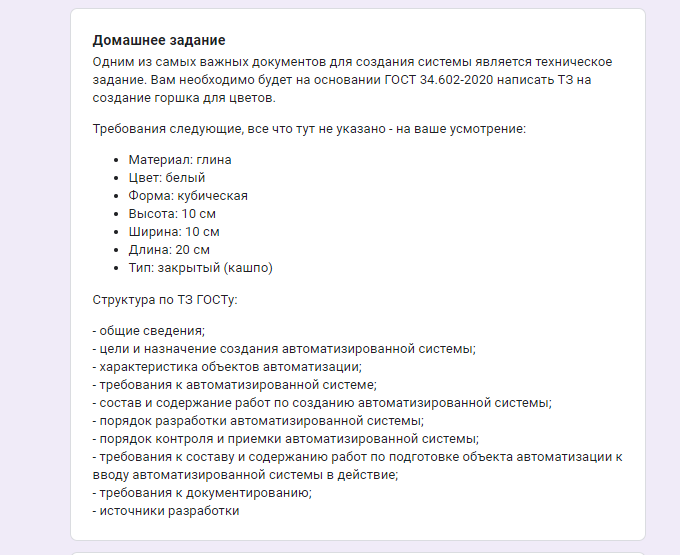
\includegraphics[width=0.7\textwidth]{изображение_2024-04-28_164154076.png}
        \caption{Задание на создание ТЗ \url{https://docs.google.com/forms/d/e/1FAIpQLSec8tqC1iCkZIwaH8GV5b6Uu8Gy_oZmZ3_r0x1xmOJQZL-JjQ/viewform}}
        \label{fig:first}
    \end{subfigure}    
    \qquad
    \begin{subfigure}{0.7\textwidth}
        \centering
        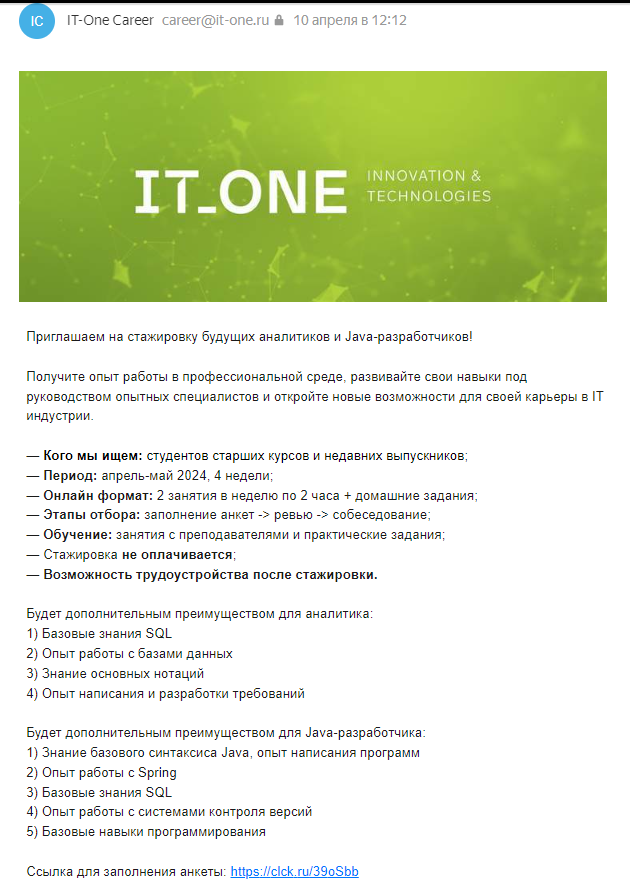
\includegraphics[width=0.7 \textwidth]{изображение_2024-04-28_164324326.png}
        \caption{Условия стажировки}
        \label{fig:second}
    \end{subfigure}    
    \caption{Материал к 1-й части}
    \label{fig:enter-label}
\end{figure}

\subsection{К секции 2}
\subsubsection{Вид глины} \label{sec:at1}
Характеристики:
\begin{itemize}
    \item GE221IMP Белая глина R\&B (10 кг)
    \item Глина содержит 20\% шамота фракции 0-0,125 мм
    \item Температура обжига 1000-1280°С
    \item Усадка при сушке     5 \%
    \item Усадка при обжиге    5 \%
    \item Влагопоглощение      1 \%
    \item КТР 20-400 °C         $44*10^-7$
    \item КТР 20-500 °C         $54*10^-7$
    \item КТР 20-500 °C         $64*10^-7$
\end{itemize}
Стоимость: 289 рублей за кг

Продукт: \url{https://ceramistam.ru/catalog/glina_frantsiya/ge221imp_belaya_glina_r_b_10_kg/#desc}
\subsubsection{Технические вычисления для объекта}
\label{sec:at2}
Горшок имеет форму параллелепипеда с одной отсутствующей гранью $bc$. Исходя из этого общая формула объёма материала в уже готовом изделии: $$V_0=2*D_0*(ac+ab+(\frac{bc}{2}))$$.
При подстановке мы получаем $V_0 = 1600 \text{sm}^3$;
Дополнительно подсчитаем потерю объёма при производстве: $$V_1 = \frac{V_0}{(1-\text{Потеря})^2} \approx 1773\text{sm}^3$$
Потеря в квадрате из-за усадки при сушке и обжиге. $V_1$ - расход материала при иделаьном горшке.
$V_2 = \frac{V_1}{(1-\text{брак})}=\frac{1773}{(1-0,35)} \approx 2728\text{sm}^3$ - потери с учётом процента брака.
\subsubsection{Технические вычисления для производительности}
\label{sec:at3}
\begin{enumerate}
    \item [11.2.3.1.] Характеристики:
\begin{itemize}
    \item SNOL 80/1200
    \item Объем, л: 80
    \item Нагрев ºC: 1200
    \item Камера Ш*Д*В, мм: 400 * 400 * 500
    \item Габариты, Ш*Д*В, мм: 940 * 980 * 1570
    \item Мощность, кВт: 7,5
    \item Напряжение, В: 380
    \item Вес, кг: 248
\end{itemize}
Продукт: \url{https://labor-snol.ru/catalog/promyshlennye-elektropechi-snol/snol-801200}
    \item [11.2.3.2.] Подсчёт вместимости
    Примем 2,5 сантиметра за отступ между заготовками, тогда:
    $$V=\frac{2*(D_0+2,5)*(ac+ab+(\frac{bc}{2}))}{(1-\text{Потеря})^2} \approx 4000\text{sm}^3$$
    
    Что соответствует 4 кубическим дециметрам. 80 литров есть 80 куб. дециметров, а значит вместительность достигает вплоть до 20 горшков за одну процедуру в одной печи. Однако, такое количество горшков не будет эффективным с точки зрения обжига. В качестве минимальной производительности, минимальным объёмом будет служить пример с полкой для схожей по размерам печи\footnote{Пример на сайте \url{https://portalkeramiki.ru/index.php/experience/statii/171-firing-ceramics}}, тогда сделаем корректировку минимального числа горшков до 10.
    Как время для изготовления горшков можно взять 6 часов (два обжига).
\end{enumerate}
\section{Согласование Технического Задания}
\begin{flushright} % сдвигает содержимое окружения вправо
Заказчик: Компания \verb|IT_ONE|, в лице
\begin{tabular}{p{.5\textwidth}} % делает таблицу из одной колонки шириной в половину текста
Должность: \hrulefill \\ % \hrulefill делает линию до конца строки
Имя сотрудника: \hrulefill \\
Подпись: \hrulefill \\
М.П.
\end{tabular}
\vspace{3em}
%\rule{\textwidth}{.3mm}

Исполнитель: Головизнин Д.И., в лице
\begin{tabular}{p{.5\textwidth}} % делает таблицу из одной колонки шириной в половину текста
Должность: \hrulefill \\ % \hrulefill делает линию до конца строки
Имя сотрудника: \hrulefill \\
Подпись: \hrulefill \\
М.П.
\end{tabular}
\end{flushright}
\end{document}